\documentclass{standalone}
\usepackage{tikz}

\begin{document}
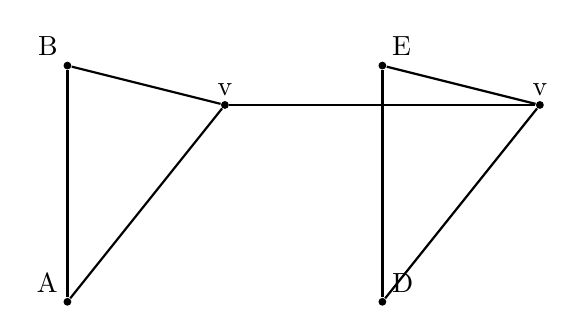
\begin{tikzpicture}[scale=2]

% Define styles for nodes and edges
\tikzset{
    vertex/.style={circle, fill=black, inner sep=1pt},
    edge/.style={thick}
}

% First Triangle
\node[vertex] (A) at (-1,-0.5) {};
\node[vertex] (B) at (-1,1) {};
\node[vertex] (C) at (0,0.75) {};

\draw[edge] (A) -- (B);
\draw[edge] (B) -- (C);
\draw[edge] (C) -- (A);

% Second Triangle
\node[vertex] (D) at (1,-0.5) {};
\node[vertex] (E) at (1,1) {};
\node[vertex] (F) at (2,0.75) {};

\draw[edge] (D) -- (E);
\draw[edge] (E) -- (F);
\draw[edge] (F) -- (D);

% Edge connecting the two triangles
\draw[edge] (C) -- (F);

% Labeling the vertices
\node[above left] at (A) {A};
\node[above left] at (B) {B};
\node[above] at (C) {v};

\node[above right] at (D) {D};
\node[above right] at (E) {E};
\node[above] at (F) {v};

\end{tikzpicture}
\end{document}